\documentclass[10pt,pdf,hyperref={unicode}]{beamer}
\usepackage{amsmath}
\usepackage[utf8]{inputenc}
\usepackage[english,russian]{babel}
\usepackage{amsfonts}
\usepackage{amsfonts,amssymb}
\usepackage{amssymb}
\usepackage{latexsym}
\usepackage{euscript}
\usepackage{enumerate}
\usepackage{graphics}
\usepackage{graphicx}
\usepackage{geometry}
\usepackage{wrapfig}

\usepackage{bbm}

\righthyphenmin=2



\usepackage[backend=biber,style=gost-numeric,sorting=none]{biblatex}
\addbibresource{../common/my.bib}
\addbibresource{../common/notmy.bib}


\usepackage{amsthm}
\theoremstyle{definition}
\newtheorem{llemma}{Лемма}
\newtheorem{ttheorem}[llemma]{Теорема}
\newtheorem{eexample}[llemma]{Пример}
\newtheorem{property}[llemma]{Свойство}
\newtheorem{remark}[llemma]{Замечание}
\newtheorem{ccorollary}{Следствие}[llemma]
\newtheorem{ddefinition}{Определение}[llemma]


%\usetheme{Antibes}
\usefonttheme{professionalfonts} % using non standard fonts for beamer
\usefonttheme[onlymath]{serif} % default family is serif
%\usepackage{fontspec}
%\setmainfont{Liberation Serif}
\begin{document}

\begin{frame}
	\frametitle{Основные определения}

	$\mathfrak{M}$~--- множество таких подмножеств
	$
		M = \{M_1, M_2, ... \}\subset \mathbb{R}^2
	$,
	что
	$
		|M_i - M_j|\in\mathbb{N}
	$
	для всех $i$, $j$, где $\mathbb{N}$~--- множество натуральных чисел
	и $|M_i - M_j|$~--- расстояние между точками $M_i$ и $M_j$.

	\begin{ttheorem}[П. Эрд\"{e}ш, 1945]
		\label{thmErdos}
		Всякое бесконечное подмножество $M\in\mathfrak{M}$
		содержится в некоторой прямой $L\in\mathbb{R}^2$.
	\end{ttheorem}

	\vspace{2em}

	Для заданного $n\in\mathbb{N}$ обозначим через $\mathfrak{M}_n$
	множество таких $M\in\mathfrak{M}$, что
	$|M|=n$ и $M \not\subset L$ для любой прямой $L \subset\mathbb{R}^2$.

	\begin{ttheorem}
		\label{thm:power_exist}
		Для любого $n\in\mathbb{N}$ выполнено $\mathfrak{M}_n\neq\varnothing$.
	\end{ttheorem}

\end{frame}


\begin{frame}
	\frametitle{Основные определения}

	$|M|$~--- мощность $M$, т.е. количество точек в множестве $M$.

	\begin{ddefinition}
		Диаметр:
		\begin{equation*}
			\operatorname{diam} M = \max_{A,B\in M} |A-B|
			,
		\end{equation*}
		где $|A-B|$~--- обычное евклидово расстояние между точками $A$ и $B$.
	\end{ddefinition}


	\begin{ddefinition}[Кемнитц, 1988]
		Характеристикой множества $M\in\mathfrak{M}_n$ называется свободное от квадратов
		число $p$, такое, что площадь любого треугольника $ABC$, где $A,B,C\in M$,
		соизмерима с $\sqrt{p}$.
	\end{ddefinition}

	\vspace{2em}

	Если $S\in\mathfrak{M}_n$, $H \subset S$, $H\in\mathfrak{M}_{p}$, $p<n$,
	то
	\begin{equation*}
		|H| < |S|, \quad \operatorname{diam} H \leq \operatorname{diam} S, \quad \operatorname{char} H = \operatorname{char} S
		.
	\end{equation*}

\end{frame}


\begin{frame}
	\frametitle{Оценки на диаметр~\cite{our-vmmsh-2018}}
	Предыдущая оценка (2016):

	\begin{ttheorem}
		Для всех $n \geq 3$, $M\in\mathfrak{M}$
		выполнено
		$
			\operatorname{diam} M \geq \dfrac{1}{8} \cdot |M|
			.
		$
	\end{ttheorem}

	\vspace{2em}

	\begin{ttheorem}
		Для всех $n \geq 4$, $M\in\mathfrak{M}$
		\begin{equation*}
			\operatorname{diam} M \geq \frac{55^2}{56^2} \cdot 0.3584 \cdot |M|
			>
			0.3457 \cdot |M|
			.
		\end{equation*}
	\end{ttheorem}


	\begin{ttheorem}
		Для достаточно больших $n$ диаметр любого множества $M\in\mathfrak{M}_n$ не менее $\frac{3}{8}n$.
	\end{ttheorem}

\end{frame}


\begin{frame}
	\frametitle{Связь с другими проблемами~\cite{our-vmmsh-2018}}

	Установлена связь исследуемой проблемы с проблемой упаковки точек в квадрат
	(packing points in the square),
	т.е. отыскания наибольшего числа $\varphi_k$, такого,
	что в единичном квадрате нельзя разместить $k$ точек так,
	чтобы расстояние между любыми двумя точками было не менее $\varphi_k$.
\end{frame}


\begin{frame}
	\frametitle{Частные случаи~\cite{our-vmmsh-2018}}

	\begin{ttheorem}
		\label{prop:edge_one}
		Пусть $M\in\mathfrak{M}_n$
		что для некоторых $M_1, M_2 \in M$ выполнено $|M_1 - M_2| = 1$.
		Тогда все точки из $M$, кроме одной, лежат на прямой $M_1 M_2$.
	\end{ttheorem}
\end{frame}

\begin{frame}
	\frametitle{Примеры множеств, найденных на ЭВМ~\cite{our-pmm-2018}}
	\begin{equation*}
		\sqrt{p}/q * \{ (x_1,y_1), ..., (x_n, y_n)  \}
		:=
		\left\{ \left(\frac{x_1}{q},\frac{y_1\sqrt{p}}{q}\right), ..., \left(\frac{x_n}{q},\frac{y_n\sqrt{p}}{q}\right)  \right\}
		%.
	\end{equation*}

	\center
	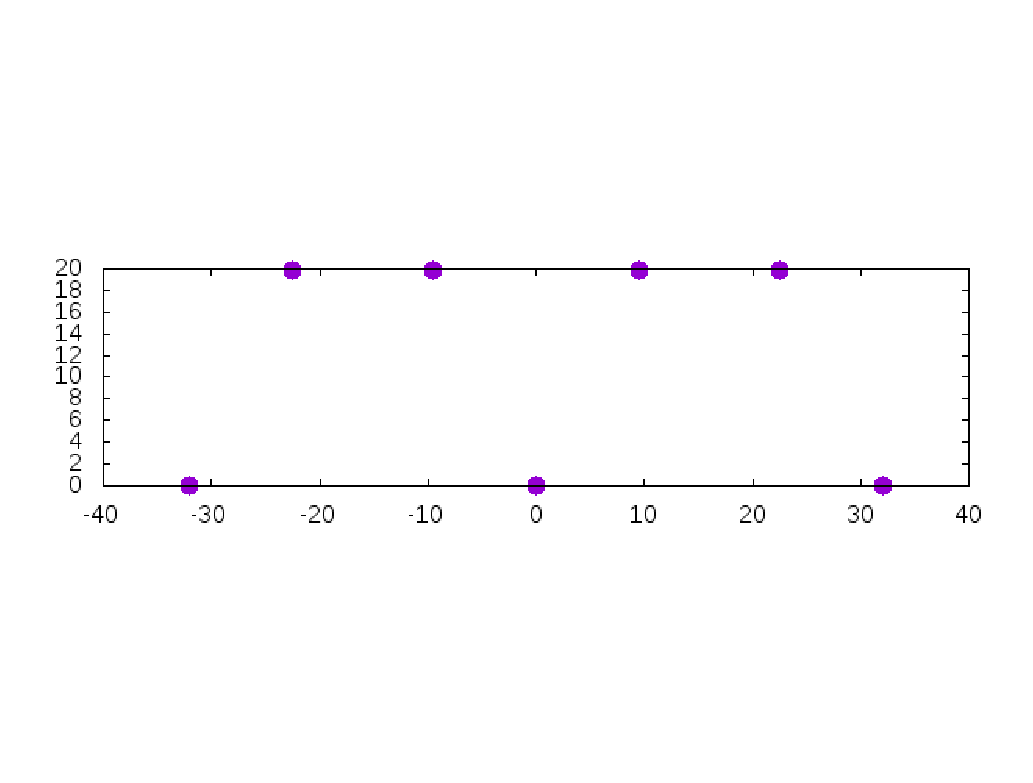
\includegraphics[width=\linewidth,trim={1 100 1 100},clip=true]{Avdeev_7_64_1538484861024.eps}


	$
	M=\sqrt{7}/2 *
	\{
	( \pm64 , 0),
	( \pm45 , 15),
	( \pm19 , 15),
	( 0 , 0)
	\}
	$,
	\\
	$\operatorname{diam} M = 64$,
	$|M| = 7$.


\end{frame}



\begin{frame}
	\frametitle{Примеры множеств, найденных на ЭВМ~\cite{our-pmm-2018}}

	\center
	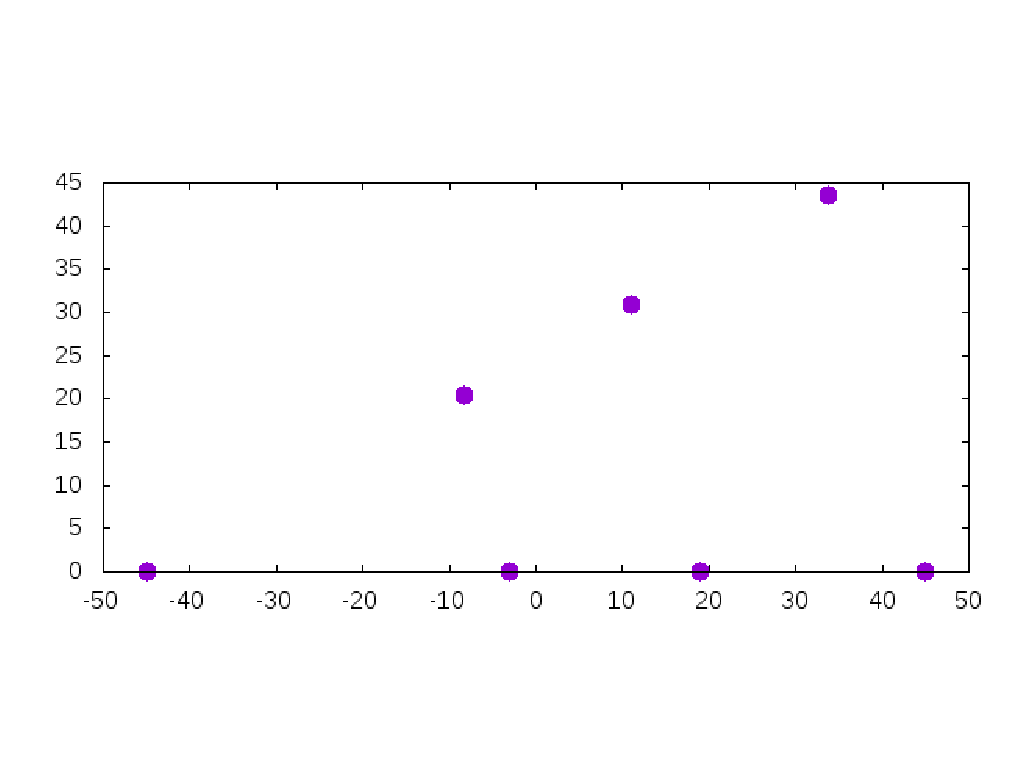
\includegraphics[width=\linewidth,trim={0 50 0 50},clip=true]{Avdeev_7_90_1538485007759.eps}


	$
	M=
	\sqrt{15}/4 *
	\{
	( \pm180 , 0),
	( 135 , 45),
	( -33 , 21),
	( 44 , 32),
	( 76 , 0),
	( -12 , 0)
	\}
	$,
	\\
	$\operatorname{diam} M = 90$,
	$|M| = 7$.


\end{frame}



\begin{frame}
	\frametitle{Примеры множеств, найденных на ЭВМ~\cite{our-pmm-2018}}

	\center
	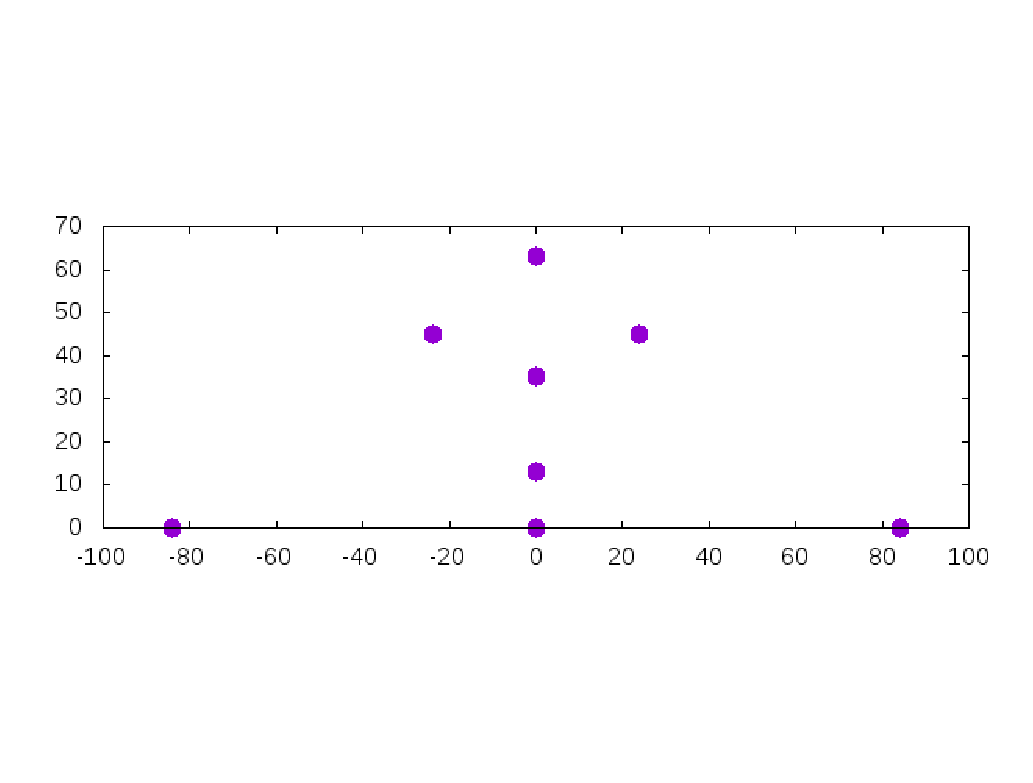
\includegraphics[width=\linewidth,trim={0 50 0 50},clip=true]{Avdeev_8_168_1538490487450.eps}


	$
	M=
	\sqrt{1}/1 *
	\{
	( \pm84 , 0),
	( \pm24 , 45),
	( 0 , 63),
	( 0 , 13),
	( 0 , 35),
	( 0 , 0)
	\}
	$,
	\\
	$\operatorname{diam} M = 168$,
	$|M| = 8$.


\end{frame}



%\begin{frame}
%	\frametitle{Примеры множеств, найденных на ЭВМ~\cite{our-ped-2018}}
%
%	\begin{columns}[onlytextwidth,T]
%		\column{0.3\linewidth}
%
%			$
%			M = \sqrt{70}/79 *
%			\{
%			$\\$
%			( \pm6241 , 0),
%			$\\$
%			( -873 , -528),
%			$\\$
%			( 2093 , 408),
%			$\\$
%			( 4838 , 138),
%			$\\$
%			( -3275 , 936),
%			$\\$
%			( -1872 , 798),
%			$\\$
%			( 5265 , 96),
%			$\\$
%			( -2299 , 840),
%			$\\$
%			( 873 , 528)
%			\}
%			$,
%			\\~\\
%			$\operatorname{diam} M = 158$,
%			$|M| = 10$.
%
%		\column{0.7\linewidth}
%			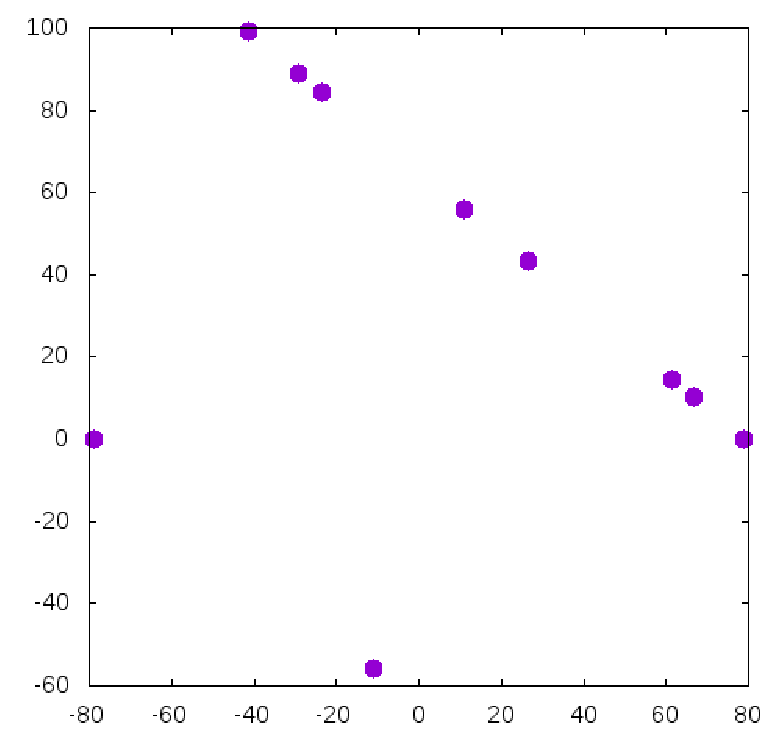
\includegraphics[width=\linewidth]{Avdeev_10_158_1538485325776.eps}
%
%    \end{columns}
%\end{frame}



\begin{frame}
	\frametitle{Примеры множеств, найденных на ЭВМ~\cite{our-ped-2018}}

		\center
		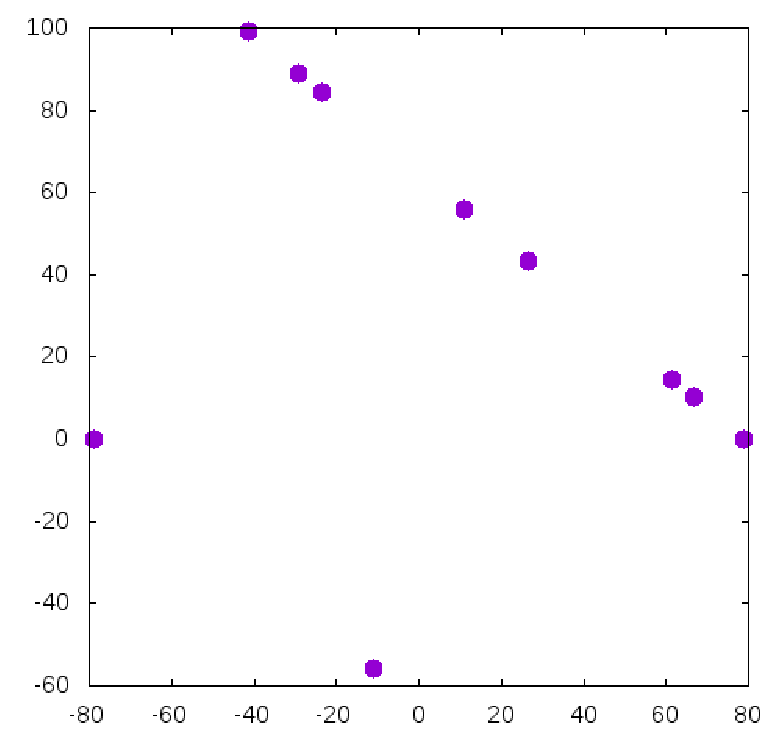
\includegraphics[width=0.6\linewidth]{Avdeev_10_158_1538485325776.eps}

			$
			M = \sqrt{70}/79 *
			\{
			( \pm6241 , 0),
			( -873 , -528),
			( 2093 , 408),
			( 4838 , 138),
			$ $
			( -3275 , 936),
			( -1872 , 798),
			( 5265 , 96),
			( -2299 , 840),
			( 873 , 528)
			\}
			$,
			$\operatorname{diam} M = 158$,
			$|M| = 10$.



\end{frame}


%%%%%%%%%%%%%%%%%%%%%%%%%%%%%%%%%%%%%%%

\begin{frame}
	\frametitle{Опубликованные работы}
	\printbibliography{}
\end{frame}

\begin{frame}
	\huge\centering
	Спасибо за внимание
\end{frame}

\end{document}
